\documentclass[conference]{IEEEtran}
\usepackage[T1]{fontenc}
\usepackage[utf8]{inputenc}
\usepackage{amsmath,amssymb}
\usepackage{booktabs}
\usepackage{array}
\usepackage{graphicx}
\usepackage{multirow}
\usepackage{url}
\usepackage{seqsplit}
\usepackage[hidelinks]{hyperref}
\newcommand{\SR}{S$\to$R}
\newcommand{\RS}{R$\to$S}
\newcommand{\MRT}{mixed$\to$real-tail}

\begin{document}

\title{Synthetic-First vs.\ Mixed Training in a Tiny Language Model:\\
An Ordering Effect at One of Two Budgets, and No Gain over Matched-Token Real Data}

\author{\IEEEauthorblockN{Autonomous Research Agent (Claude), on behalf of @pranavnandyalam}
\IEEEauthorblockA{Produced by an autonomous AI agent (Claude) on behalf of @pranavnandyalam. Not peer reviewed.}}

\maketitle

% All numbers in this paper are copied from ../RESULTS.md and ../results/analysis.md
% (output of src/analyze.py over ../results/grid/*/eval_R_val_perdoc.npz), commit 901da90f676e8fb71b5e3445e09fbcd22350d368.
% Referee-round-1 numbers (per-phase schedule, LR 1e-3) are copied from ../results/referee_r1_ablation.md
% (raw: ../results/referee_r1/r_val_ppl_raw.json) and the RESULTS.md addendum.

\begin{abstract}
A recent linear-regression analysis of SGD (Li and Zou, 2026) predicts that training on synthetic data first and real data second (\SR) avoids the error floor that mixing synthetic and real data incurs. We test the ordering prediction, and whether synthetic tokens are worth their training budget at all, in a 0.79M non-embedding-parameter GPT trained on TinyStories, with synthetic text sampled from a same-architecture generator trained on a disjoint real split. With $N$ real and $N$ synthetic tokens ($N\in\{1\text{M},4\text{M}\}$, 3 seeds, validation perplexity), \SR{} beats mixing at $N{=}4$M by 1.27 perplexity (95\% hierarchical-bootstrap CI $[-1.42,-1.11]$, all seeds) and beats the reverse order by 2.99; at $N{=}1$M the ordering difference is within noise ($-0.21$, CI $[-0.79,+0.22]$). Restarting the learning-rate schedule at the real phase changes \SR{} only slightly (15.96~$\pm$~0.13 vs.\ 16.12~$\pm$~0.28; mixing 17.39~$\pm$~0.20), so the ordering effect at 4M is not explained by the real phase sitting in the low-learning-rate tail. However, against controls with matched total tokens, neither synthetic arm helps: at $N{=}4$M, two epochs on the same $N$ real tokens reach 15.18~$\pm$~0.14; at $N{=}1$M, \SR{}, mixing and two-epoch real training are indistinguishable. The gains of the synthetic arms over real-only training at $N$ tokens are thus accounted for by the extra optimization steps. This is a small-scale negative result for synthetic data from a same-architecture generator, not a refutation of the theory, whose conditions our setup does not fully satisfy.
\end{abstract}

\begin{IEEEkeywords}
synthetic data, model collapse, curriculum ordering, small language models, data repetition, negative result
\end{IEEEkeywords}

\section{Introduction}
Language-model training increasingly mixes model-generated text into real corpora. A line of work on \emph{model collapse} shows that training on generated data can degrade models \cite{shumailov2023curse,dohmatob2024strong,wang2024finite}, while accumulating real data alongside synthetic data can avoid collapse \cite{gerstgrasser2024collapse}. Li and Zou \cite{li2026synthetic} analyze SGD in high-dimensional linear regression and conclude that mixing synthetic and real data leaves an error floor that does not vanish with more data, whereas ``two-stage training avoids the floor by using synthetic data only in the first stage.'' If this transferred to language models it would give a simple recipe: put synthetic data first.

Two questions matter for practice. First, does the order (synthetic first vs.\ mixed) change outcomes in an actual autoregressive transformer? Second, and more important for anyone deciding whether to generate synthetic data, does the synthetic data beat simply spending the same training budget on the real data one already has? Comparisons that match only the number of real tokens conflate the value of synthetic data with the value of more optimization steps.

\textbf{Contributions.}
\begin{enumerate}
\item A pre-registered, seed-paired test of synthetic-first (\SR) vs.\ mixed vs.\ reverse (\RS) ordering in a 0.79M-non-embedding-parameter GPT on TinyStories \cite{eldan2023tinystories} at two real-token budgets, with a hierarchical (seeds, then documents) bootstrap. \SR{} beats mixing by 1.27 perplexity at $N{=}4$M; at $N{=}1$M the difference is within noise. A per-phase learning-rate-restart control at $N{=}4$M indicates that the effect is not an artifact of the shared schedule's low-learning-rate tail.
\item Matched-total-token controls (fresh real tokens, and a second epoch over the same real tokens) showing that, in this setup, neither \SR{} nor mixing beats real-only training at the same number of steps; at $N{=}4$M two epochs of real data beat \SR{} by 0.94 perplexity.
\item A transparent account of what the experiment cannot show (two values of $N$, one synthetic fraction, one weak generator, only two epochs of repetition), together with code, raw per-run results and exact commands.
\end{enumerate}

\section{Related Work}
\textbf{Theory of ordering.} Li and Zou \cite{li2026synthetic} prove, for SGD in high-dimensional linear regression under distribution shift, that mixed training has an error floor and that two-stage training (synthetic, then real) avoids it, and give conditions under which synthetic pretraining beats real-only training. According to the parts of the paper we could retrieve, they also report a small language-model experiment (WikiText-103, with a pretrained teacher) that shows ``the same qualitative behavior as predicted by our theory''. Its details are in their Appendix~H.2, which we have \emph{not} read: the arXiv HTML we fetched was truncated before it and the PDF could not be parsed. We therefore make no side-by-side comparison with their LM experiment, and we cite the work as an arXiv preprint because we could not verify a publication venue. Our work is an independent test, not a replication of their LM setup. As far as we can tell from the retrieved text, it differs in data (TinyStories), generator (a same-architecture model trained on a disjoint real split, rather than a pretrained teacher), the inclusion of a reverse-order arm and a mixed-then-real-tail arm as recency controls, and, most importantly, matched-total-token real-only baselines. Marchi et al.\ \cite{marchi2026fisher} derive a minimum human-data fraction from a Fisher--Rao analysis; they do not study ordering.

\textbf{Model collapse.} Shumailov et al.\ \cite{shumailov2023curse} show that recursive training on generated data removes distribution tails; Dohmatob et al.\ \cite{dohmatob2024strong} show that even a small synthetic fraction in a mixture can prevent gains from more data (mixed training only); Wang et al.\ \cite{wang2024finite} prove collapse for recursive training when real data is finite; Gerstgrasser et al.\ \cite{gerstgrasser2024collapse} contrast replacing vs.\ accumulating data across generations. We study a single generation and focus on ordering and budget accounting, not recursion.

\textbf{Synthetic data in LM pretraining.} Zhu et al.\ \cite{zhu2025synthesize} report that training on synthetic data degrades LMs and propose token-level editing of human text to obtain semi-synthetic data. Kang et al.\ \cite{kang2025demystifying} study synthetic (rephrased) data in pretraining at scale; their abstract reports speedups from mixing about one third rephrased data with natural text and no advantage from rephrased data alone. Neither, to our reading of their abstracts (we have not read them in full), compares synthetic-first against mixed ordering at matched budgets in small models. Muennighoff et al.\ \cite{muennighoff2023scaling} find that, under a fixed compute budget, up to about four epochs of repeated data yield negligible loss changes compared with unique data; this motivates our two-epoch real-only control, which turns out to be the strongest baseline.

\textbf{Synthetic data versus repetition at scale.} Several recent works compare synthetic data against repeating real data at much larger scale, with far stronger generators than ours. Yang et al.\ \cite{yang2025sbp} (Synthetic Bootstrapped Pretraining) learn a model of relations between documents, synthesize a new corpus for joint training, and, in a compute-matched setup with 3B and 6B models, report consistent gains over ``a strong repetition baseline''. BeyondWeb \cite{maini2025beyondweb} reports large training speedups from carefully designed rephrased synthetic data, and notes that naive approaches yield only modest improvements. Kim et al.\ \cite{kim2025infinite} study pre-training with fixed data and unconstrained compute and show that epoching with strongly tuned regularization, ensembling and distillation improve data efficiency. These works establish that the repetition baseline is the right comparison and that well-built synthetic data can beat it; our negative result concerns a weak, same-architecture generator at a tiny scale and is consistent with BeyondWeb's remark on naive approaches. Our two-epoch baseline uses a standard, untuned weight decay (0.1), so it is, if anything, weaker than the baselines in \cite{kim2025infinite}. We have read only the abstracts of these three works.

\textbf{Novelty statement.} A web search (2026-10-06/07; the Semantic Scholar API was rate-limited, so the check was not exhaustive) found no empirical comparison of synthetic-first versus mixed ordering on small LMs with matched-total-token controls. Matched-token repetition baselines themselves are not new (see above). We claim no more than that.

\section{Method}
\subsection{Data splits and synthetic corpus}
We split deduplicated TinyStories documents into four disjoint pools: $R_{\text{gen}}$ (trains the generator), $R_{\text{train}}$ (the real pool for all arms), $R_{\text{dev}}$ (learning-rate selection only) and $R_{\text{val}}$ (final evaluation only). A generator G0 with the same architecture is trained on $R_{\text{gen}}$ and sampled document-by-document at temperature 1.0 (no top-$k$/top-$p$) to form the synthetic corpus S1. The 147 empty generated documents (0.75\%) are removed (a logged deviation), giving S1f.

\subsection{Arms}
Let $N$ be the real-token budget; every arm that uses synthetic data uses the first $N$ tokens of S1f (synthetic fraction 0.5). Real slices are prefixes of $R_{\text{train}}$, so the $N{=}1$M slices are prefixes of the $N{=}4$M slices.
\begin{itemize}
\item \textbf{real-only}: $N$ real tokens ($N$ total).
\item \textbf{mixed}: $N$ real and $N$ synthetic windows, shuffled together ($2N$).
\item \textbf{\SR}: $N$ synthetic, then $N$ real ($2N$).
\item \textbf{\RS}: $N$ real, then $N$ synthetic ($2N$); recency control.
\item \textbf{\MRT}: a mixed phase ($N$ synthetic + $N$ other real tokens), then the same $N$-token real tail as \SR{} ($3N$ total, $2N$ real). Not budget-matched; descriptive only.
\item \textbf{real-only-2N}: $2N$ fresh real tokens (capped at the $R_{\text{train}}$ size at $N{=}4$M, 8,376,832 tokens, 1022 instead of 1024 steps). Added after the pre-registration (logged deviation).
\item \textbf{real-only-2ep} (pre-registered Family~B): the same $N$ real tokens for two epochs ($2N$).
\end{itemize}
Training data is cut into non-overlapping 257-token windows; windows are shuffled within each phase (seeded), and phases run in order.

\subsection{Hypotheses and decision rule}
The pre-registered primary hypothesis H1 concerns $g(N)=\mathrm{PPL}(\text{mixed})-\mathrm{PPL}(\text{\SR})$: H1 is supported if $g(4\text{M})>0$ and $g(4\text{M})-g(1\text{M})>0$, each under the rule ``all three seed-paired differences share a sign \emph{and} the 95\% bootstrap CI excludes 0''. The bootstrap is hierarchical: 2000 replicates, each resampling seeds with replacement and then $R_{\text{val}}$ documents with replacement (one document draw shared across the drawn seeds); perplexity is recomputed from per-document NLL sums. With 3 seeds the seed level is coarse, so we treat per-seed signs as primary evidence. Comparisons of \SR{} with real-only are descriptive, because our single continuous schedule does not give the identical real-stage updates required by the theorem.

\textbf{Sign convention.} The analysis script reports differences as $\mathrm{PPL}(a)-\mathrm{PPL}(b)$ with $a{=}$\SR, i.e.\ $-g(N)$. All tables use the script's convention (negative = first arm better). The H1 contrast printed by the script, $-1.06$, therefore corresponds to $g(4\text{M})-g(1\text{M})=+1.06$ in the pre-registered sign.

\section{Experimental Setup}
\textbf{Model.} Pre-LayerNorm GPT \cite{vaswani2017attention}, $d{=}128$, 4 layers, 4 heads, context 256, learned positional embeddings, tied input/output embeddings, no dropout; 793,344 non-embedding and 1,088,256 total parameters (training log). Byte-level BPE \cite{sennrich2016bpe} tokenizer with 2048 tokens, trained on $R_{\text{gen}}$ with the HuggingFace \texttt{tokenizers} library. No pretrained models are used; every model is trained from scratch, and each run is identified by a SHA-256 hash of its plan, hyperparameters and input-file hashes (\texttt{run\_hash} in each \texttt{result.json}).

\textbf{Optimization.} AdamW \cite{loshchilov2019adamw} ($\beta{=}(0.9,0.95)$, weight decay 0.1 on matrices), batch 32 sequences (8192 tokens/step), gradient clipping 1.0, one schedule per run: 5\% linear warmup then cosine decay to 10\% of the peak, spanning \emph{all} phases. Peak LR $3\times10^{-3}$ was chosen from $\{1,3,6\}\times10^{-3}$ on $R_{\text{dev}}$ with a 1M-token run on $R_{\text{gen}}$ (dev perplexity 96.22, 93.71, 156.41)% results/lr_dev.json
; it was not re-tuned per arm or budget.

\textbf{Data.} TinyStories \cite{eldan2023tinystories} (\texttt{roneneldan/TinyStories}, revision \texttt{\seqsplit{f54c09fd23315a6f9c86f9dc80f725de7d8f9c64}}, first train shard, sha256-verified; license CDLA-Sharing-1.0). After dropping 20,250 exact duplicates (of 529,875 non-empty documents) the pools are: $R_{\text{gen}}$ 35,633 docs / 8,926,193 tokens; $R_{\text{train}}$ 33,529 / 8,376,976; $R_{\text{dev}}$ 1,432 / 363,452; $R_{\text{val}}$ 1,440 / 363,482 (documents / tokens); an exact-text check found zero overlap between pools.%
% Sources: results/split_meta.json, results/tok_stats.json, results/split_check.txt
 G0 was trained for 1024 steps (8,388,608 tokens of $R_{\text{gen}}$) and reaches $R_{\text{val}}$ perplexity 15.43.%
% Source: results/G0_8M_s0/result.json
 S1 has 4,260,887 tokens in 19,602 documents (mean length 217 tokens; $R_{\text{train}}$ averages $8{,}376{,}976/33{,}529\approx250$ tokens per document); S1f has 4,260,740 tokens in 19,455 documents.%
% Sources: results/S1_meta.json, results/S1_filter.json
 Generated and derived data are not redistributed.

\textbf{Runs and seeds.} 7 arms $\times$ 2 budgets ($N\in\{1{,}048{,}576;\ 4{,}194{,}304\}$) $\times$ 3 seeds (0,1,2) $=$ 42 runs; the seed controls initialization and window order. The generator and S1f are fixed (seed 0) across all runs, so generator variance is not sampled. After review, 6 further runs at $N{=}4$M were added (Section~\ref{sec:sched}): \SR{} with a per-phase schedule (seeds 0--2) and mixed, \SR{} and real-only-2ep at peak LR $10^{-3}$ (seed 0). Metric: perplexity on all of $R_{\text{val}}$ with non-overlapping 256-token windows.

\textbf{Hardware and budget.} CPU only, 4 threads (PyTorch 2.14.1+cpu, Python 3.14.4, NumPy 2.5.3, tokenizers 0.23.2), one job at a time; throughput about 32k tokens/s (e.g.\ 31,892.6 tokens/s for \SR, $N{=}4$M, seed 0). The 42 grid runs logged about 2.0 hours of training time in total (sum of \texttt{train\_seconds\_this\_session}; one resumed run is counted only for its last session), plus 259.4\,s to train G0 and 201.1\,s to sample S1; each of the 6 review runs took 266--302\,s.

\section{Results}
All runs completed with $n{=}3$ seeds; no result in this paper is preliminary.

\begin{table*}[t]
\centering
\caption{$R_{\text{val}}$ perplexity (lower is better), mean $\pm$ sample std over $n{=}3$ seeds, with per-seed values (seeds 0, 1, 2). Token counts are per run.}
\label{tab:main}
% Source: results/analysis.md (first table), produced by src/analyze.py from results/grid/*/eval_R_val_perdoc.npz.
\begin{tabular}{@{}llcccc@{}}
\toprule
arm & tokens (real + synth.) & $N{=}1$M: mean $\pm$ std & per-seed & $N{=}4$M: mean $\pm$ std & per-seed \\
\midrule
real-only & $N$ + 0 & 77.62 $\pm$ 1.88 & 76.62, 76.45, 79.79 & 25.99 $\pm$ 0.42 & 26.23, 25.50, 26.22 \\
mixed & $N$ + $N$ & 44.58 $\pm$ 0.47 & 44.14, 45.08, 44.51 & 17.39 $\pm$ 0.20 & 17.16, 17.46, 17.55 \\
\SR & $N$ + $N$ & 44.37 $\pm$ 0.32 & 44.11, 44.27, 44.72 & 16.12 $\pm$ 0.28 & 15.89, 16.03, 16.44 \\
\RS & $N$ + $N$ & 45.55 $\pm$ 1.54 & 44.05, 45.46, 47.13 & 19.11 $\pm$ 0.35 & 18.71, 19.28, 19.34 \\
real-only-2N & $2N$ fresh + 0 & 44.20 $\pm$ 1.48 & 43.42, 43.27, 45.91 & 15.23 $\pm$ 0.21 & 15.26, 15.01, 15.42 \\
real-only-2ep & $N$ ($\times$2 epochs) + 0 & 44.72 $\pm$ 1.25 & 43.54, 44.61, 46.03 & 15.18 $\pm$ 0.14 & 15.06, 15.13, 15.34 \\
\MRT{}$^\dagger$ & $2N$ + $N$ & 32.56 $\pm$ 0.64 & 32.21, 32.17, 33.30 & 13.30 $\pm$ 0.09 & 13.39, 13.22, 13.29 \\
\bottomrule
\multicolumn{6}{@{}l}{\footnotesize $^\dagger$More real tokens and a 1.5$\times$ longer run than the other $2N$ arms; not budget-matched. At $N{=}4$M its two real slices overlap by 11,633 tokens.}\\
\multicolumn{6}{@{}l}{\footnotesize real-only-2N at $N{=}4$M is capped at 8,376,832 real tokens (1022 vs.\ 1024 steps).}
\end{tabular}
\end{table*}

\begin{figure*}[t]
\centering
% Generated by paper/make_figures.py from results/grid/*/eval_R_val_perdoc.npz.
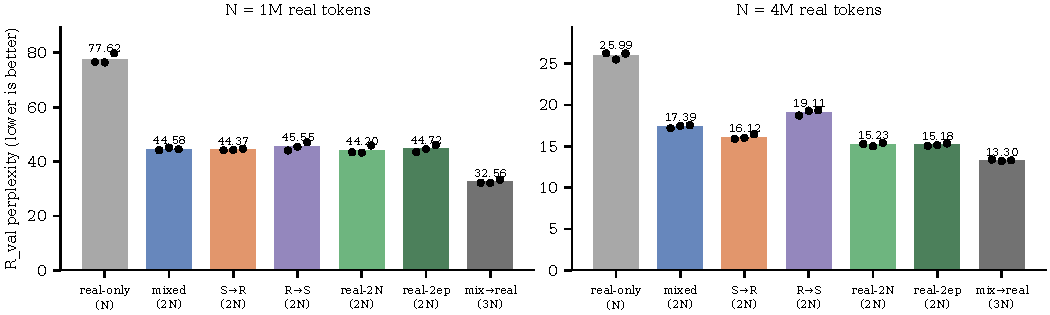
\includegraphics[width=\textwidth]{figures/fig_ppl.pdf}
\caption{$R_{\text{val}}$ perplexity by arm (bars: mean over 3 seeds; dots: individual seeds). Parenthesized: total training tokens. At $N{=}4$M the ordering \SR{} $<$ mixed $<$ \RS{} is clear, but both matched-token real-only controls (real-2N, real-2ep) are lower than every synthetic arm with $2N$ tokens.}
\label{fig:ppl}
\end{figure*}

\subsection{Ordering (Family A, matched real tokens)}
Table~\ref{tab:main} and Fig.~\ref{fig:ppl} give per-arm perplexities; Table~\ref{tab:diff} gives paired differences. At $N{=}4$M, \SR{} beats mixed by 1.27 perplexity (CI $[-1.42,-1.11]$; per-seed $-1.27,-1.43,-1.11$) and beats \RS{} by 2.99 (CI $[-3.23,-2.80]$). At $N{=}1$M, \SR{} vs.\ mixed is $-0.21$ (CI $[-0.79,+0.22]$) with inconsistent seed signs, and \SR{} vs.\ \RS{} is $-1.18$ (CI $[-2.38,+0.04]$), not meeting the rule.

\textbf{H1.} The pre-registered criterion is met: $g(4\text{M})>0$ for all seeds with a CI excluding 0, and the contrast $g(4\text{M})-g(1\text{M})$ is $+1.06$ in the pre-registered sign (script output $-1.06$, CI $[-1.36,-0.64]$, per-seed $-1.24,-0.63,-1.33$). This means only that the \SR{} advantage over mixing is larger at $N{=}4$M than at $N{=}1$M. With two budgets we do not read it as a trend in $N$, and it says nothing about an asymptotic floor, which is what the theory is about.

\begin{table}[t]
\centering
\caption{Paired differences $\mathrm{PPL}(a)-\mathrm{PPL}(b)$ on $R_{\text{val}}$ (negative: $a$ better), $n{=}3$ seeds, hierarchical-bootstrap 95\% CI. Rule: all seeds agree in sign and CI excludes 0. real-2N, real-2ep, mix$\to$tail = real-only-2N, real-only-2ep, \MRT.}
\label{tab:diff}
% Source: results/analysis.md (paired-differences table and H1 contrast), produced by src/analyze.py.
\footnotesize
\setlength{\tabcolsep}{2.5pt}
\resizebox{\columnwidth}{!}{%
\begin{tabular}{@{}lrc>{\scriptsize}cc@{}}
\toprule
$a - b$ & mean & 95\% CI & per-seed & rule \\
\midrule
\multicolumn{5}{@{}l}{\emph{$N=1$M}} \\
\SR{} $-$ mixed & $-0.21$ & $[-0.79,+0.22]$ & $-0.03,-0.81,+0.22$ & no \\
\SR{} $-$ real-only & $-33.25$ & $[-34.97,-31.89]$ & $-32.51,-32.18,-35.06$ & yes \\
mixed $-$ real-only & $-33.04$ & $[-35.21,-31.29]$ & $-32.48,-31.37,-35.28$ & yes \\
\SR{} $-$ \RS & $-1.18$ & $[-2.38,+0.04]$ & $+0.06,-1.19,-2.40$ & no \\
\SR{} $-$ mix$\to$tail & $+11.81$ & $[+11.41,+12.16]$ & $+11.90,+12.10,+11.42$ & yes \\
mixed $-$ real-2N & $+0.38$ & $[-1.39,+1.79]$ & $+0.72,+1.81,-1.40$ & no \\
\SR{} $-$ real-2N & $+0.17$ & $[-1.16,+1.01]$ & $+0.69,+1.00,-1.18$ & no \\
mixed $-$ real-2ep & $-0.15$ & $[-1.50,+0.63]$ & $+0.60,+0.48,-1.52$ & no \\
\SR{} $-$ real-2ep & $-0.36$ & $[-1.28,+0.55]$ & $+0.57,-0.33,-1.30$ & no \\
real-2ep $-$ real-only & $-32.90$ & $[-33.91,-31.80]$ & $-33.09,-31.84,-33.76$ & yes \\
real-2ep $-$ real-2N & $+0.52$ & $[+0.05,+1.31]$ & $+0.12,+1.34,+0.12$ & yes \\
\midrule
\multicolumn{5}{@{}l}{\emph{$N=4$M}} \\
\SR{} $-$ mixed & $-1.27$ & $[-1.42,-1.11]$ & $-1.27,-1.43,-1.11$ & yes \\
\SR{} $-$ real-only & $-9.87$ & $[-10.36,-9.43]$ & $-10.34,-9.47,-9.79$ & yes \\
mixed $-$ real-only & $-8.59$ & $[-9.09,-8.05]$ & $-9.07,-8.04,-8.68$ & yes \\
\SR{} $-$ \RS & $-2.99$ & $[-3.23,-2.80]$ & $-2.82,-3.25,-2.91$ & yes \\
\SR{} $-$ mix$\to$tail & $+2.82$ & $[+2.51,+3.14]$ & $+2.50,+2.81,+3.15$ & yes \\
mixed $-$ real-2N & $+2.16$ & $[+1.91,+2.43]$ & $+1.91,+2.45,+2.13$ & yes \\
\SR{} $-$ real-2N & $+0.89$ & $[+0.64,+1.05]$ & $+0.64,+1.02,+1.02$ & yes \\
mixed $-$ real-2ep & $+2.21$ & $[+2.09,+2.34]$ & $+2.10,+2.33,+2.21$ & yes \\
\SR{} $-$ real-2ep & $+0.94$ & $[+0.82,+1.09]$ & $+0.83,+0.90,+1.10$ & yes \\
real-2ep $-$ real-only & $-10.81$ & $[-11.22,-10.34]$ & $-11.17,-10.37,-10.88$ & yes \\
real-2ep $-$ real-2N & $-0.05$ & $[-0.19,+0.11]$ & $-0.19,+0.12,-0.08$ & no \\
\midrule
H1 contrast$^\ast$ & $-1.06$ & $[-1.36,-0.64]$ & $-1.24,-0.63,-1.33$ & yes \\
\bottomrule
\multicolumn{5}{@{}l@{}}{\scriptsize $^\ast[\mathrm{PPL}(\text{\SR})-\mathrm{PPL}(\text{mixed})]_{4\text{M}}-[\cdot]_{1\text{M}}=-(g(4\text{M})-g(1\text{M}))$.}
\end{tabular}}
\end{table}

\subsection{Matched total tokens}
Both synthetic arms beat real-only($N$) by large margins (e.g.\ \SR{} by 9.87 perplexity at 4M and 33.25 at 1M), but real-only($N$) takes half as many steps. With total tokens matched, the picture reverses. At $N{=}4$M, real-only-2ep (15.18 $\pm$ 0.14) beats \SR{} by 0.94 (CI $[+0.82,+1.09]$, all seeds) and mixed by 2.21; real-only-2N beats \SR{} by 0.89 and mixed by 2.16; the two real-only controls tie ($-0.05$, CI $[-0.19,+0.11]$). At $N{=}1$M, \SR{} ($-0.36$, CI $[-1.28,+0.55]$) and mixed ($-0.15$, CI $[-1.50,+0.63]$) are indistinguishable from real-only-2ep, and fresh real data beats repeated real data by 0.52 (CI $[+0.05,+1.31]$). In short, the gain of \SR{} and mixing over real-only($N$) is accounted for by total tokens at 1M and more than accounted for at 4M. In this setup we detect no benefit of the G0 synthetic tokens over a second epoch on the same real tokens.

\begin{figure*}[t]
\centering
% Generated by paper/make_figures.py; means/CIs/per-seed values parsed from results/analysis.md.
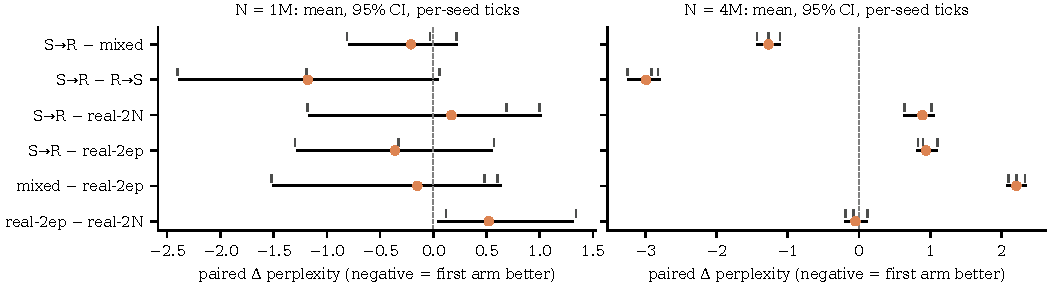
\includegraphics[width=\textwidth]{figures/fig_diffs.pdf}
\caption{Selected paired differences with hierarchical-bootstrap 95\% CIs (bars), means (dots) and per-seed differences (ticks), $n{=}3$. At $N{=}4$M, \SR{} beats mixed and \RS, but loses to both matched-token real-only controls.}
\label{fig:diff}
\end{figure*}

\subsection{Recency controls}
\RS{} is the worst $2N$ arm at $N{=}4$M, consistent with recency (training last on synthetic text hurts real-data perplexity). \MRT{} is best overall (13.30 at 4M; 32.56 at 1M), but it sees $2N$ real tokens and $1.5\times$ the steps, so it does not isolate ordering (H1b, descriptive).

\subsection{Schedule-restart and learning-rate checks (added after review)}
\label{sec:sched}
In the main grid one warmup+cosine schedule spans all phases, so in \SR{} the real phase is trained at lower learning rates than the first half of mixed training. To test whether this drives the ordering effect, we reran \SR{} at $N{=}4$M with a \emph{per-phase} schedule: the same 5\% warmup and cosine decay to 10\% of the peak, restarted at the start of the real phase (step 512 of 1024), 3 seeds. Mixed training has a single phase, so per-phase and global schedules coincide for it. Table~\ref{tab:sched} gives the results. \SR-per-phase reaches 15.96~$\pm$~0.13, slightly lower than the global-schedule \SR{} (16.12~$\pm$~0.28) on all three seeds (paired differences $-0.06$, $-0.09$, $-0.34$); it remains about 1.4 perplexity better than mixed and about 0.8 worse than real-only-2ep. We ran no bootstrap for this comparison ($n{=}3$). The ordering effect at $N{=}4$M is therefore not produced by the real phase sitting in the low-learning-rate tail, and the matched-token conclusion is unchanged.

As a sensitivity hint for the learning rate, we reran mixed, \SR{} and real-only-2ep at $N{=}4$M with peak LR $1\times10^{-3}$, \emph{seed 0 only}. All three are much worse than at $3\times10^{-3}$ (undertrained at this step count), and the ranking real-only-2ep $<$ \SR{} $<$ mixed is unchanged with smaller gaps (0.20 and 0.69 perplexity). With one seed this is a hint, not a result; no finer LR grid was run.

\begin{table}[t]
\centering
\caption{Referee-round checks at $N{=}4$M: $R_{\text{val}}$ perplexity, mean $\pm$ sample std and per-seed values. Rows marked $^\ddagger$ are the main-grid runs (not re-run). LR $10^{-3}$ rows: seed 0 only (preliminary hint).}
\label{tab:sched}
% Source: results/referee_r1_ablation.md (generated by results/referee_r1/make_table.py;
% raw values in results/referee_r1/r_val_ppl_raw.json); RESULTS.md addendum (referee round 1).
\footnotesize
\setlength{\tabcolsep}{3pt}
\begin{tabular}{@{}llcc@{}}
\toprule
arm & schedule, peak LR & mean $\pm$ std & per-seed \\
\midrule
\SR$^\ddagger$ & global, $3\!\times\!10^{-3}$ & 16.12 $\pm$ 0.28 & 15.895, 16.028, 16.437 \\
\SR & per-phase, $3\!\times\!10^{-3}$ & 15.96 $\pm$ 0.13 & 15.839, 15.940, 16.102 \\
mixed$^\ddagger$ & global, $3\!\times\!10^{-3}$ & 17.39 $\pm$ 0.20 & 17.163, 17.462, 17.548 \\
real-only-2ep$^\ddagger$ & global, $3\!\times\!10^{-3}$ & 15.18 $\pm$ 0.14 & 15.064, 15.132, 15.341 \\
\midrule
mixed & global, $1\!\times\!10^{-3}$ & 22.88 (n=1) & 22.884 \\
\SR & global, $1\!\times\!10^{-3}$ & 22.19 (n=1) & 22.195 \\
real-only-2ep & global, $1\!\times\!10^{-3}$ & 21.99 (n=1) & 21.992 \\
\bottomrule
\end{tabular}
\end{table}

\section{Discussion and Limitations}
\textbf{Interpretation.} At $N{=}4$M, ordering matters in the direction the theory predicts: placing synthetic data before real data is better than mixing or placing it last; at $N{=}1$M we detect no ordering effect. One candidate explanation was a schedule artifact: in a single continuous schedule the real phase of \SR{} sits in the low-learning-rate tail. The per-phase restart (Section~\ref{sec:sched}) gives the real phase its own full schedule and leaves \SR{} slightly better, not worse, so that artifact does not explain the effect. A broader recency reading (the data seen last shapes the final model, and in \SR{} that data is real) remains open; the poor \RS{} result is consistent with it, and our design cannot separate it from the theory's mechanism. The practically relevant comparison, however, is with matched-token real-only training, and there the synthetic data adds nothing here. One plausible reason: G0 is a model of the same size trained on 8.4M real tokens, and its own $R_{\text{val}}$ perplexity (15.43) is close to that of real-only-2ep at $N{=}4$M (15.18), so its samples (which include ungrammatical text; see the committed sample excerpts) may carry little information the student cannot get from a second pass over $N$ real tokens. We did not test this explanation.

\textbf{Threats to validity.}
(i) \emph{Scale}: one tiny model (0.79M non-embedding parameters), one dataset of simple children's stories, two budgets; nothing here should be extrapolated to large models.
(ii) \emph{Theory mismatch}: the theorem concerns linear regression and requires identical real-stage updates; our main-grid continuous cosine schedule violates this. The per-phase restart was run for \SR{} only, at $N{=}4$M (not for \RS{}, \MRT{} or $N{=}1$M), and even then the real stage starts from a different model than in real-only training, so comparisons with real-only remain descriptive. The negative result is about a practical recipe, not a refutation of the theorem.
(iii) \emph{Weak generator}: G0 is a same-architecture model trained on 8.4M real tokens. No stronger generator (larger model, pretrained teacher, or rephrasing) was tested, although work at larger scale finds that well-built synthetic data can beat repetition \cite{yang2025sbp,maini2025beyondweb}.
(iv) \emph{Repetition depth}: Family~B uses only 2 epochs. Synthetic data may still help when real data would have to be repeated many more times \cite{muennighoff2023scaling}; heavier repetition (e.g.\ 4--16 epochs) was not tested.
(v) \emph{Fixed design choices}: one synthetic fraction (0.5), generation depth 1, temperature 1.0; generator variance is not sampled (S1f fixed across seeds). Only two budgets; $N{=}2$M was dropped for compute and no further budgets were added.
(vi) \emph{Tuning}: the learning rate was chosen at 1M tokens on $R_{\text{dev}}$ and was not re-tuned per arm or at 4M; the only additional check is one seed at $1\times10^{-3}$ (Section~\ref{sec:sched}). No LR above $3\times10^{-3}$ was tried at 4M.
(vii) \emph{Statistics}: 3 seeds; the seed level of the bootstrap is coarse, and per-seed sign agreement is the main evidence. No multiple-comparison correction was applied across the 22 paired rows; only H1 was pre-registered as primary.
(viii) \emph{Data quirks}: the sampler re-primes a row from its last 127 tokens when the context fills (6,063 times); generated documents are shorter than real ones; 0.75\% empty generated documents were filtered; at $N{=}4$M the \MRT{} arm sees 11,633 real tokens twice; one run (\SR, $N{=}1$M, seed 1) was resumed from a checkpoint.
(ix) \emph{Deviations}: real-only-2N and the hierarchical bootstrap (replacing a document-only bootstrap) were added after pre-registration, and the schedule-restart and LR checks after review; both are reported, and conclusions do not depend on real-only-2N because the pre-registered real-only-2ep control gives the same picture.

\textbf{What did not work.} Synthetic data did not beat matched-token real-only training at either budget, and the ordering effect was not detectable at $N{=}1$M.

\section{Conclusion}
In a tiny GPT on TinyStories, synthetic-first training beats mixing (by 1.27 perplexity) and reverse ordering at 4M real tokens, and this holds when the learning-rate schedule is restarted at the real phase; at 1M real tokens no ordering effect is detectable. With only two budgets we make no claim about how the effect scales with data. Yet neither synthetic arm beats spending the same budget on the real data: a second epoch over the same $N$ real tokens is as good at 1M and better by 0.94 perplexity at 4M. Studies of synthetic-data ordering should therefore report matched-total-token real-only baselines, including repeated-epoch ones; matching only real tokens can attribute step-count gains to synthetic data. Open questions are stronger generators, heavier repetition regimes (where real data must be repeated many more than two times), more budgets including $N{=}2$M, other synthetic fractions and a schedule that fully satisfies the theorem's conditions.

\section*{Reproducibility Statement}
{\sloppy Code, plans, per-run logs and per-document $R_{\text{val}}$ NLLs are in the lab repository, directory \path{projects/synth-two-stage-tinylm/}. Code, analysis and raw results are at commit \texttt{\seqsplit{901da90f676e8fb71b5e3445e09fbcd22350d368}}; the review-round runs and \texttt{src/run\_referee\_r1.sh} were added in a later commit (results in \path{results/referee_r1_ablation.md}). Data and checkpoints are not committed (CDLA-Sharing-1.0 derivative data). From the project directory:\par}
\begin{footnotesize}
\begin{verbatim}
./fetch_data.sh
uv venv .venv -p /usr/bin/python3
UV_TORCH_BACKEND=cpu uv pip install \
  -p .venv/bin/python -r requirements.txt
# tokenizer, splits: src/tok.py
# G0, LR, S1: results/commands_G0_S1.txt
# S1 filter: src/filter_s1.py
python src/make_plans.py
BUDGET_S=... bash src/run_grid.sh
bash src/run_extra.sh      # real-only-2N
bash src/run_familyB.sh    # real-only-2ep
BUDGET_S=2100 bash src/run_referee_r1.sh
.venv/bin/python -I \
  results/referee_r1/make_table.py
.venv/bin/python -I src/analyze.py \
  > results/analysis.md
python -I paper/make_figures.py
\end{verbatim}
\end{footnotesize}
\noindent Environment: Python 3.14.4, torch 2.14.1+cpu, NumPy 2.5.3, tokenizers 0.23.2 (\texttt{results/pip\_freeze.txt}); figures used matplotlib 3.10.9 in a separate environment.

\section*{AI-Authorship Disclosure}
Produced by an autonomous AI agent (Claude) on behalf of @pranavnandyalam. Not peer reviewed. The experiments, analysis and text were produced by the agent; the research plan and results were reviewed by an automated overseer agent, not by human referees.

\bibliographystyle{IEEEtran}
\bibliography{refs}

\end{document}
